\chapter{Experimentos}\label{cap:experimentos}

\section{Detalles de experimentación}
El principal experimento consto en replicar los resultados de Bansal \cite{bansal2018zero}, ya que no se pudo encontrar el código en la red. Tratamos de ser lo mas fiel posible a su definición, pero fue necesario asumir muchos detalles y probar con distintos valores hasta llegar a un valor aproximado a lo que reportan. Por otro lado, no realizamos exactamente sus experimentos, ya que esto no aportaría nada nuevo. Así que, se decidió analizar sus resultados y solo replicar los que consideramos indispensable y que seria un buen punto de partida. Por ejemplo, los experimentos con clases de fondo, no obtuvieron buenos resultados, en comparación con los que no la utiliza. Es por esto que no consideramos realizaros. Ademas, cuestionamos sus métricas y se analizaron nuevas mediciones para poder obtener una forma de comparar con otros trabajos. También, se analizaron los resultados de los modelos para Zero-shot convencional y generalizado.

Por un error de interpretación con las métricas de Bansal, nos llevo a probar distintas configuraciones como, que generador de propuestas o que CNN utilizar. Por mucho tiempo, nos enfocamos en encontrar las combinaciones de parámetros, que maximice las métricas. Pero gracias a esto obtuvimos unas mejoras significantes a los valores reportados.

Ahora definamos la metodológica de evaluación. El primer paso es generar propuestas para cada imagen, a cada propuesta se le extrae el vector de características visuales, luego se rescala la imagen al tamaño de la capa de entrada y se utiliza el modelo entrenado para inferir el vector de características semánticas. Después, se calcula la similitud coseno con los vectores semánticos de todas las clases o solo las invisibles, dependiendo si se quiere evaluar ZSD o ZSDG. Aquella clase que obtenga el mayor puntaje es asignada a la propuesta. También, se guarda la puntuación como la confianza de predicción.  Por ultimo, se agrupan todas las propuestas que se tengan asignada la misma clase y se corre un algoritmo de supresión no máxima. NMS elimina las predicciones repetidas y solo nos deja la mejor propuestas. Al final obtenemos como resultado un conjunto de propuestas, sus clases y su respectivo puntaje. \\
 

\begin{table}[]
	\centering
	\resizebox{12.5cm}{!} {
	\begin{tabular}{|l|c|r|r|r|c|r|}
		\hline
		\textbf{}                     & \multicolumn{4}{c|}{\textbf{Edge Boxes}}                                                                                                   & \multicolumn{2}{c|}{\textbf{Selective Search}}               \\ \hline
		\textbf{Algoritmo}            & \multicolumn{4}{c|}{\textbf{-}}                                                                                                            & \textbf{Single}         & \multicolumn{1}{c|}{\textbf{Fast}} \\ \hline
		\textbf{Numero de propuestas} & \textbf{100}                 & \multicolumn{1}{c|}{\textbf{500}} & \multicolumn{1}{c|}{\textbf{1000}} & \multicolumn{1}{c|}{\textbf{5000}} & \textbf{$\approx$ 1000} & \multicolumn{1}{c|}{\textbf{100}}  \\ \hline
		Tiempo promedio (s)           & \multicolumn{1}{r|}{0.11}    & 0.11                              & 0.12                               & 0.12                               & \multicolumn{1}{r|}{}   &                                    \\ \hline
		Propuetas Totales             & \multicolumn{1}{r|}{4415244} & 22050071                          & 43802935                           & 161809194                          & \multicolumn{1}{r|}{}   &                                    \\ \hline
		Propuestas con IOU $> 0.5$    & \multicolumn{1}{r|}{86233}   & 133942                            & 155584                             & 194891                             & \multicolumn{1}{r|}{}   &                                    \\ \hline
	\end{tabular}
}
	\caption{Resultados de correr los distintos algoritmos de propuestas de regiones en los datos de entrenamiento. El numero de propuestas verdaderas es 261258.}
	\label{tab:edgeVSselct}
\end{table}
El numero de propuestas es un parámetro clave en esta etapa, por que gran cantidad de ellas, hace que tome mucho tiempo correr las métricas y proporciona una gran cantidad de . Por otra parte si no se generan las suficiente, puede que muchos objetos sean ignorados. Es por esto que se probaron dos algoritmos (Edge Boxes y Selective Search) y muchas combinaciones de parámetros. Para cada imagen de entrenamiento se corrió el generador de propuestas y se calculo el tiempo y la cantidad de cuadros verdaderos que tenían un IoU $> 0.5$. Este experimento, como se puede observar en el Cuadro \ref{tab:edgeVSselct}, arrojo que la mejor opción es usar Edge-boxes al igual que en el trabajo de Bansal. En cuanto tiempo y numero de propuestas totales resulto mejor usar 500 propuestas ya que al aumentar este numero no se genera mejoras significativas y se hace mas costoso en cuanto a tiempo innecesariamente.\\

Otro punto que se decidió analizar fue la CNN. Lo que se quiere aquí es que la red sea capas de asocias las caracteristicas visuales de objetos similares, y diferenciar los elementos de distinta naturaleza. En otras palabras, el espacio resultante tiene que distribuirse de tal manera que por ejemplo las imágenes de los animales estén muy cerca y a su ves alejado de vehículos o electrodomésticos, pero también tiene que mantener una separación entre los distintos animales como perro y gato. Bansal en su trabajo utiliza \textbf{Inception ResNet V2}, lo cual nos genero curiosidad y se decidió probar con otra CNN \textbf{VGG16}, y de esta manera ver como influye en el modelo completo. Para esto se comparo miles de recuadros de 3 clases de entrenamiento, caballo, perro y camión. Por cada cuadro se genero el vector de caracteristicas visuales, luego se comparo utilizando la similitud coseno, entre las caracteristicas de caballo vs caballo, caballo vs camión y caballo vs perro. Se graficaron (Figura \ref{fig:vgg-vs-resnet}) las frecuencias de los resultados para cada CNN. Como se esperaba la similitud entre entre animales es mas grande que con un vehiculo. También, se observo que para \textbf{Inception ResNet V2} existe una mayor separación entre clases. Por esta razón se espera un mejor rendimiento que \textbf{VGG16}.\\

% para generar tablas de latex
\begin{figure}
	\centering
	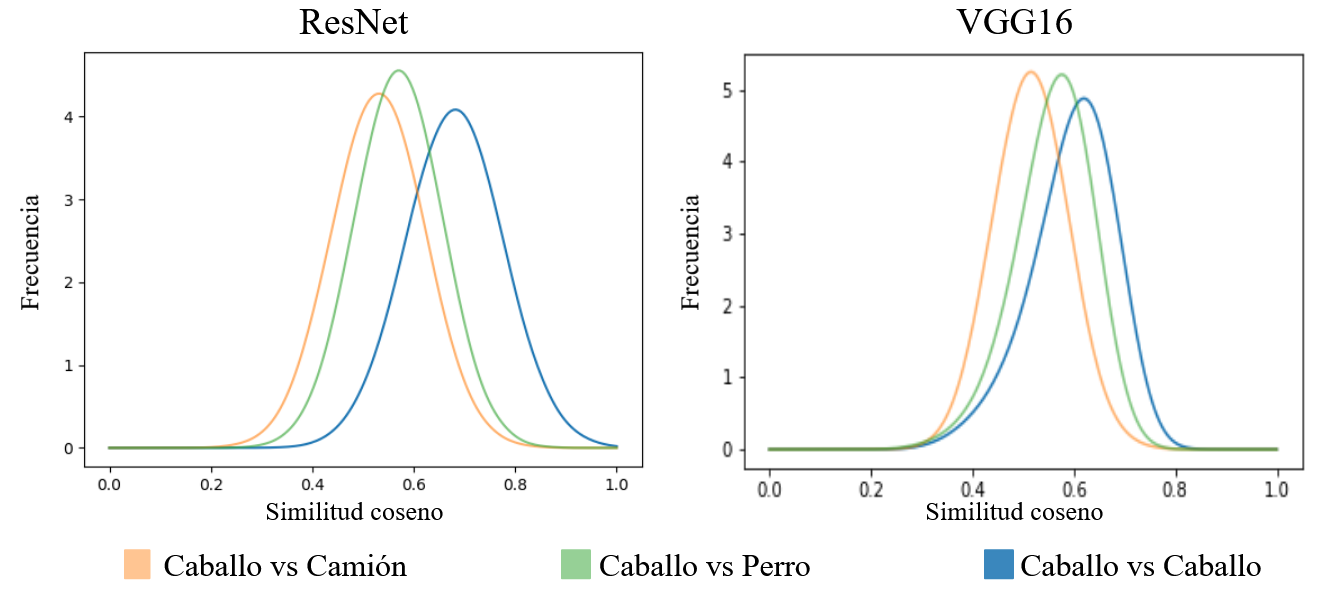
\includegraphics[width=0.8\linewidth]{img/vgg-vs-resnet}
	\caption{Frecuencia de la similitud coseno de los vectores de caracteristicas visuales, ente la misma y distintas clases, para las CNN  \textbf{Inception ResNet V2} y \textbf{VGG16}.}
	\label{fig:vgg-vs-resnet}
\end{figure}

Las métricas mas utilizadas para medir el rendimiento de ZSD son \textbf{Recall} y \textbf{Mean Average Precision (mAP)}. Pero primero es necesario aclarar cuando una propuestas es considerada
\begin{itemize}
	\item Falso negativo (\textbf{FN}): No se obtuvo ninguna detección en absoluto, o para un cuadro delimitador verdadero el IoU $> 0.5$ y no se predijo correctamente la clase
	\item Falso positivo (\textbf{FP}): Para un cuadro delimitador verdadero, se predijo correctamente la clase pero el IoU $< 0.5$, o es un predicción duplicada, es decir, ya se marco otra con mayor IOU como \textbf{TP}.
	\item Verdadero positivo (\textbf{TP}): Para un cuadro delimitador verdadero, se obtuvo  una propuesta con un IoU $> 0.5$ y se predijo correctamente la clase.
	\item Verdadero negativo (\textbf{TN}): Esto solo tiene sentido si, se quisiera medir propuestas que no tenían un IoU $> 0.5$ con todos los cuadros verdaderos, y ademas se predijo como clase de fondo. Pero en este trabajo no es utilizada.
\end{itemize}

La \textbf{Recall}, también conocida como sensibilidad, mide la probabilidad de que los objetos verdaderos (los que se encuentran en la imagen) se detecten correctamente, viene dado por: \[Recall =\frac{TP}{FN+TP}\] En el trabajo de Bansal, calcula la Recall utilizando los falsos positivos. Es aquí donde surgió una interpretación errónea de las métricas. Sin poner en tela de juicio, si esto esta bien o mal, es claro que de esta forma solo se tiene en cuenta, los objetos que tuvieron al menos una propuesta con un IoU $> 0.5$ y el resto, quedan fuera del calculo de esta métrica. Bansal, calcula una variación denominada K@Recall, donde solo se tienen en cuentan las K mejores propuestas basándose en la confianza de la predicción y el resto son descartadas.\\

Para calcular la AP, de una clase específica por ejemplo ``persona", se calcula la curva de precision-recall, variando el umbral del IoU, luego se toma el valor medio de la precisión en todos los valores de recall. \textbf{mAP} para la detección de objetos es el promedio del AP calculado para todas las clases. Por lo general también se indica sobre que IoU se calcula, por ejemplo, mAP@0.5, o un conjunto de umbrales como mAP@[x, y]. El trabajo de Bansal reporta \textbf{mAP}, pero no indica sobre que IoU se calcula, a si que se asume que utilizo un valor de 0,5. Muchos trabajos que utilizan COCO, reportan mAP@[.5, .95], que es provista por la API del mismo conjunto de datos. Esta métrica resulta muy útil si se quiere comparar rendimientos entre distinto trabajos.

% https://www.tablesgenerator.com/ LAS
\section{Análisis de resultados}

